\documentclass[11pt, a4paper]{article}

\usepackage[margin=1in]{geometry}
\usepackage{graphicx}
\usepackage{amsmath, amssymb}
\usepackage{listings}
\usepackage{xcolor}
\usepackage{hyperref}
\usepackage{booktabs}
\usepackage{subcaption}
\usepackage{float}
\usepackage{fancyhdr}
\usepackage{enumitem}

\pagestyle{fancy}
\fancyhf{}
\fancyfoot[C]{\thepage}

\begin{document}

\fancypagestyle{no_hdr_border_rule}{
  \renewcommand{\headrulewidth}{0pt}
}
\thispagestyle{no_hdr_border_rule}

\begin{center}
    {\Large \textbf{Experiment 5 -- Report}} \\[0.2cm]
    {\large \textbf{Digital Systems and Microcontrollers (DSM)}} \\[0.1cm]
    {\normalsize International Institute of Information Technology, Hyderabad} \\[0.3cm]
\end{center}

\vspace{0.2cm}
\hrule
\vspace{0.4cm}

\noindent \textbf{Student Name 1:} Manbir Singh Judge \hfill \textbf{Roll Number:} 2026113005 \\
\noindent \textbf{Student Name 2:} Charishma Kandregula \hfill \textbf{Roll Number:} 2026112022 \\
\noindent \textbf{Table Number:} 16 \hfill \textbf{Lab Room Number:} N114 \\
\noindent \textbf{Date of Experiment:} 01/10/2026

\vspace{0.4cm}
\hrule
\vspace{0.5cm}

\vspace{1em}

\tableofcontents
\vspace{0.5cm}
\hrule
\vspace{0.8cm}

\newpage
\fancyhead[L]{Experiment 5 -- Report}

\section{Aim}

Assembly and testing of SR latch and JK flip-flop and implementation of 4-bit ripple counter using Arduino.

\section{Part A -- SR Latch}

\subsection{Aim}
Assembly and testing of SR latch.

\subsection{Components \& Equipment Required}
\begin{itemize}
    \item Digital Test Kit (DTK) -- including power supply, switches, indicator LED pairs and breadboard
    \item IC CD4001-NOR
    \item Connecting Wires
\end{itemize}

\subsection{Circuit Diagram}
Following is the circuit diagram for SR latch using 2 NOR gates:
\begin{figure}[H]
    \centering
    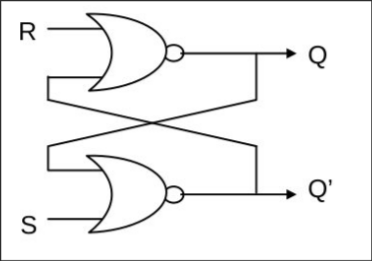
\includegraphics[width=0.3\textwidth]{circuit1.png}
    \caption{Circuit Diagram for SR Latch}
\end{figure}

\subsection{Procedure}
\begin{itemize}
    \item Place the IC CD4001 on the breadboard and verify the operation of the 4 NOR gates.
    \item Wire the circuit according to the circuit diagram (using 2 NOR gates from IC CD4001).
    \item Observe and tabulate the sequence of $Q$ and $Q'$ outputs for the following input sequence: $$SR = 10, 00, 01, 00, 10, 00, 01, 00$$
    \item Interpret the observed result and verify latch operation.
\end{itemize}

\subsection{Observations}
\begin{table}[H]
    \centering
    \caption{Outputs for Sequence of Inputs to SR Latch}
    \begin{tabular}{|cc|cc|}
        \hline
        $S$ & $R$ & $Q$ & $Q'$ \\
        \hline
        1 & 0 & 1 & 0 \\
        \hline
        0 & 0 & 1 & 0 \\
        \hline
        0 & 1 & 0 & 1 \\
        \hline
        0 & 0 & 0 & 1 \\
        \hline
        1 & 0 & 1 & 0 \\
        \hline
        0 & 0 & 1 & 0 \\
        \hline
        0 & 1 & 0 & 1 \\
        \hline
        0 & 0 & 0 & 1 \\
        \hline
    \end{tabular}
\end{table}

\subsection{Tinkercad Simulation}
\textbf{Tinkercad Link:} \href{https://www.tinkercad.com/things/1I8dcB0KGs2-dsm-experiment-5-part-a?sharecode=k30GHRaOVOH1eQkrPLMFaD09P_5DM3RhGOdXqolqq74}{\color{blue}Click here}
\begin{figure}[H]
\centering
    \centering
    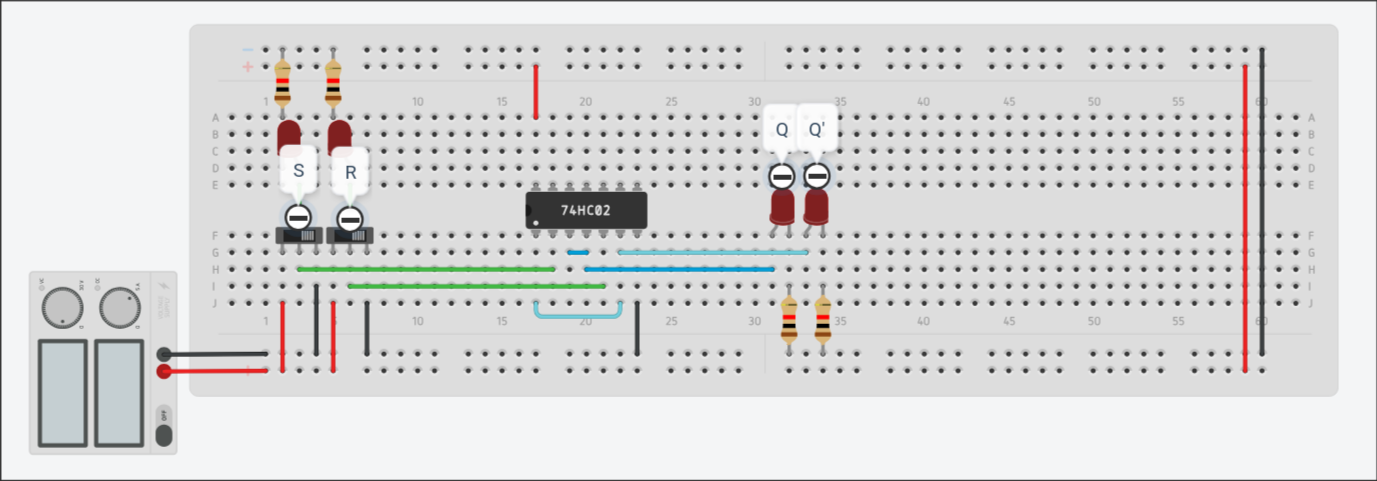
\includegraphics[width=\textwidth]{tc1.png}
    \caption{Tinkercad Simulation Screenshot}
\end{figure}

\subsection{Hardware Setup Photograph}
\begin{figure}[H]
    \centering
    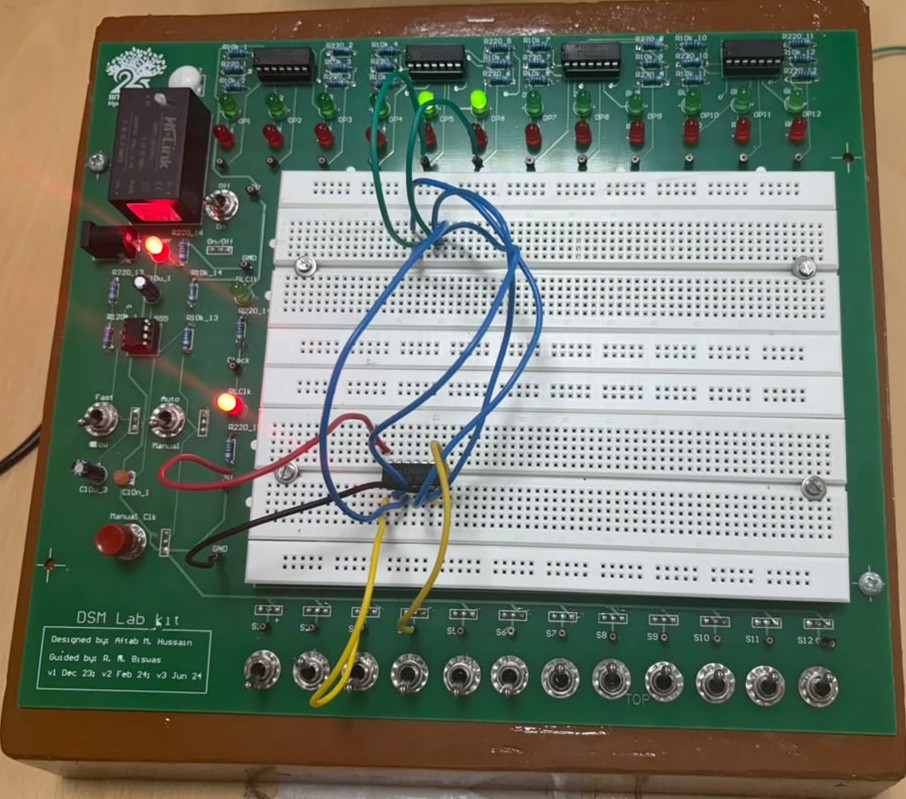
\includegraphics[width=0.6\textwidth]{lab1.jpeg}
    \caption{Physical Circuit for SR Latch}
\end{figure}

\subsection{Conclusion}
We can conclude that: 
\begin{itemize}
    \item $Q = 1$ in set state ($S = 1$ and $R = 0$).
    \item $Q = 0$ in reset state ($S = 0$ and $R = 1$). 
    \item If $S = 0$ and $R = 0$, latch holds the previous output.
\end{itemize}

\section{Part B -- JK Flip-Flop}

\subsection{Aim}
Assembly and testing of JK flip-flop.

\subsection{Components \& Equipment Required}
\begin{itemize}
    \item Digital Test Kit (DTK) -- including power supply, switches, indicator LED pairs, breadboard and clock
    \item \textbf{ICs:}
    \begin{itemize}[label=$\bullet$]
        \item 1 CD4001 -- Quad 2-input NOR
        \item 2 CD4012 -- Bi 4-input NAND
    \end{itemize}
    \item Connecting Wires
\end{itemize}

\subsection{Circuit Diagram}
Following is the circuit diagram for JK flip-flop:
\begin{figure}[H]
    \centering
    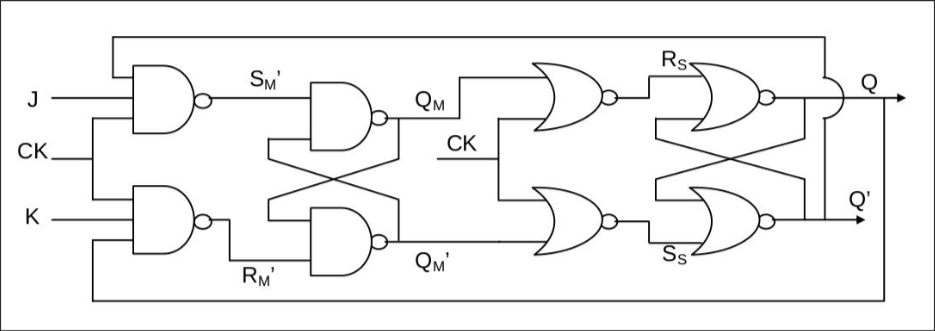
\includegraphics[width=0.8\textwidth]{circuit2.png}
    \caption{Circuit Diagram for JK flip-flop}
\end{figure}
\noindent \textbf{Implementation note:} 3-input and 2-input NAND can be made using 4-input NAND gates by setting the unused inputs to 1.

\subsection{Procedure}
\begin{itemize}
    \item Place the ICs on the breadboard and verify the operation of all gates.
    \item Wire the circuit according to the circuit diagram.
    \item Observe and tabulate the sequence of $Q$ for all combinations for $J$ and $K$ for at least 3 clock cycles.
    \item Interpret the observed result and verify flip-flop operation.
\end{itemize}

\subsection{Observations}
\begin{table}[H]
    \centering
    \caption{Observed Output Sequence of JK Flip-Flop}
    \begin{tabular}{|c|c|c|c|c|c|}
        \hline
        Clock Cycle & $J$ & $K$ & $Q_n$ & $Q_{n-1}$ & State \\
        \hline
        1  & 1 & 0 & 1 & X & \\
        2  & 1 & 0 & 1 & 1 & Set \\
        3  & 1 & 0 & 1 & 1 & \\
        \hline
        4  & 0 & 0 & 1 & 1 & \\
        5  & 0 & 0 & 1 & 1 & Hold \\
        6  & 0 & 0 & 1 & 1 & \\
        \hline
        7  & 0 & 1 & 0 & 1 & \\
        8  & 0 & 1 & 0 & 0 & Reset \\
        9  & 0 & 1 & 0 & 0 & \\
        \hline
        10 & 0 & 0 & 0 & 0 & \\
        11 & 0 & 0 & 0 & 0 & Hold \\
        12 & 0 & 0 & 0 & 0 & \\
        \hline
        13 & 1 & 1 & 1 & 0 & \\
        14 & 1 & 1 & 0 & 1 & Toggle \\
        15 & 1 & 1 & 1 & 0 & \\
        \hline
    \end{tabular}
\end{table}

\subsection{Tinkercad Simulation}
\textbf{Tinkercad Link:} \href{https://www.tinkercad.com/things/6Vp4zClkFAH-dsm-experiment-5-part-b?sharecode=s1slhPF5fHmvodEfrx09f89USW9zaUwrhkasP67lhZk}{\color{blue}Click here}
\begin{figure}[H]
\centering
    \centering
    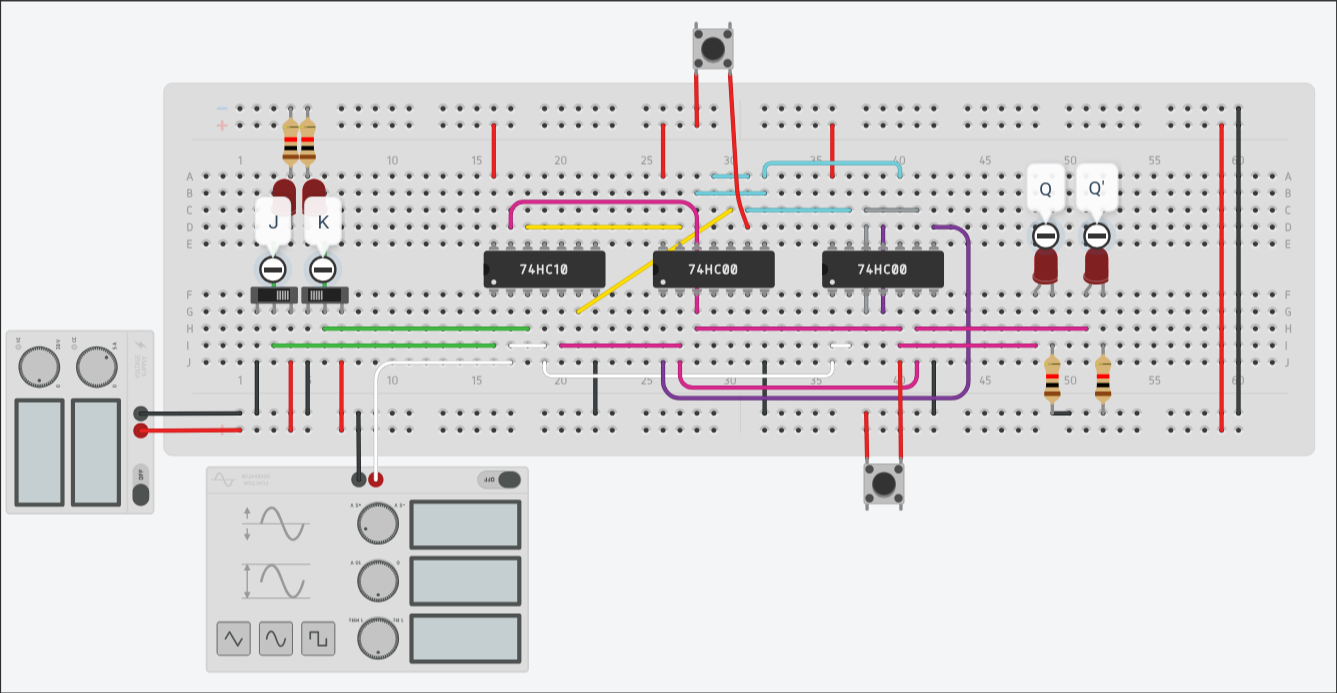
\includegraphics[width=\textwidth]{tc2.png}
    \caption{Tinkercad Simulation Screenshot}
\end{figure}

\subsection{Hardware Setup Photograph}
\begin{figure}[H]
    \centering
    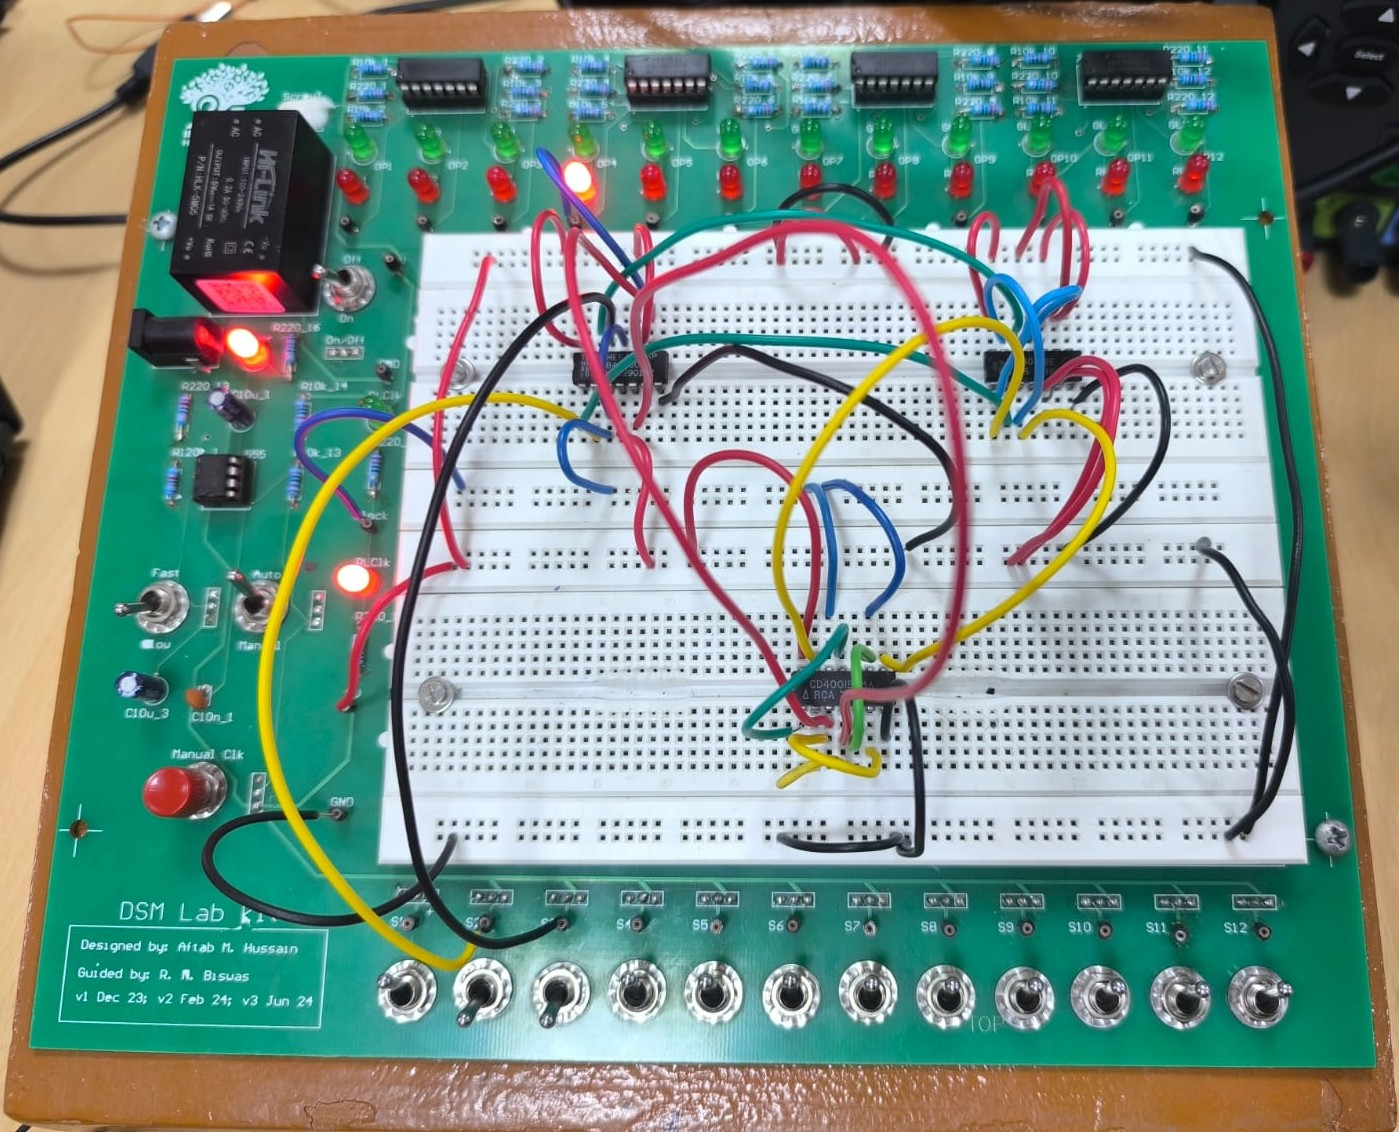
\includegraphics[width=0.6\textwidth]{lab2.jpeg}
    \caption{Physical Circuit for SR Latch}
\end{figure}

\subsection{Conclusion}
We can conclude that, following is the truth table for the JK flip-flop. Flip-flop updates for $Q_n$ to $Q_{n+1}$ each clock cycle.
\begin{table}[H]
    \centering
    \caption{Conclusive Truth Table for JK Flip-Flop}
    \begin{tabular}{|cc|c|}
        \hline
        $S$ & $R$ & $Q_{n+1}$ \\
        \hline
        0 & 0 & $Q_n$ \\
        \hline
        1 & 0 & 1 \\
        \hline
        0 & 1 & 0 \\
        \hline
        1 & 1 & $Q_n'$ \\
        \hline
    \end{tabular}
\end{table}

\section{Part C -- 4-bit Up-Down Counter}

\subsection{Aim}
To build a 4-bit up-down counter using Arudino.

\subsection{Components, Equipment \& Prerequisites Required}
\begin{itemize}
    \item Digital Test Kit (DTK) -- including power supply, switches, indicator LED pairs, breadboard and clock
    \item Arduino UNO Board
    \item USB A-to-B cable
    \item Connecting Wires
    \item Boiler-plate code for $Timer$ class in Arduino Sketch (provided in Lab Manual).
\end{itemize}

\subsection{Arduino Code}

\definecolor{vscodeBg}{rgb}{0.12, 0.12, 0.12}     
\definecolor{vscodeFg}{rgb}{0.86, 0.86, 0.86}     
\definecolor{vscodeKeyword}{rgb}{0.34, 0.61, 0.84}
\definecolor{vscodeControl}{rgb}{0.77, 0.53, 0.75}
\definecolor{vscodeString}{rgb}{0.81, 0.57, 0.47} 
\definecolor{vscodeComment}{rgb}{0.42, 0.60, 0.33}
\definecolor{vscodeNumber}{rgb}{0.71, 0.80, 0.66} 
\definecolor{vscodeLineNum}{rgb}{0.53, 0.53, 0.53}
\lstdefinestyle{customstyle}{
    backgroundcolor=\color{vscodeBg},   
    basicstyle=\ttfamily\small\color{vscodeFg},
    commentstyle=\color{vscodeComment}\itshape,
    keywordstyle=\color{vscodeKeyword}\bfseries,
    stringstyle=\color{vscodeString},
    numberstyle=\small\color{vscodeLineNum},
    breaklines=true,                 
    captionpos=b,                    
    numbers=left,                    
    numbersep=8pt,                  
    tabsize=2,
    showstringspaces=false,
    rulecolor=\color{vscodeBg}
}
\lstset{style=customstyle}

\begin{lstlisting}[language=C++, caption={Arduino Code for Part C}]
// ----------------------------
#define i0 9
#define i1 10
#define i2 11
#define i3 12

Timer t;

bool state = HIGH;

void reverseTimers() {
  	state = !state;  
    t.oscillate(i0, 500 , state, 8);
    t.oscillate(i1, 1000, state, 4);
    t.oscillate(i2, 2000, state, 2);
    t.oscillate(i3, 4000, state, 1);
}

void setup() {
    Serial.begin(9600);
  
    pinMode(i0, OUTPUT);  
    pinMode(i1, OUTPUT);  
    pinMode(i2, OUTPUT);  
    pinMode(i3, OUTPUT);
  
    t.oscillate(i0, 500 , state, 8);
    t.oscillate(i1, 1000, state, 4);
    t.oscillate(i2, 2000, state, 2);
    t.oscillate(i3, 4000, state, 1);
  
  	t.every(8000, reverseTimers);
}

void loop() {
    t.update();
}
// ----------------------------
\end{lstlisting}

\subsection{Procedure}
\begin{itemize}
    \item Connect Arduino UNO to the computer using USB A-to-B cable.
    \item Connect output pins 9-12 to indicator LED pairs on DKT.
    \item Write the above code in Arduino IDE in provided space of boiler-plate code.
    \item Compile and upload the code to Arduino.
    \item Observe and verify the up-down counting.
\end{itemize}

\subsection{Observations}
The connected indicator LED pairs were lighting up in sequence of counting of 4-bit binary numbers; up and down alternatingly.

\subsection{Tinkercad Simulation}
\textbf{Tinkercad Link:} \href{https://www.tinkercad.com/things/gxyAb7y0oft-dsm-experiment-5-lab-c?sharecode=S7CtO316aFhX94XgY7IQjC4xgW8w0_QUWpvVCA_A1LI}{\color{blue}Click here}
\begin{figure}[H]
\centering
    \centering
    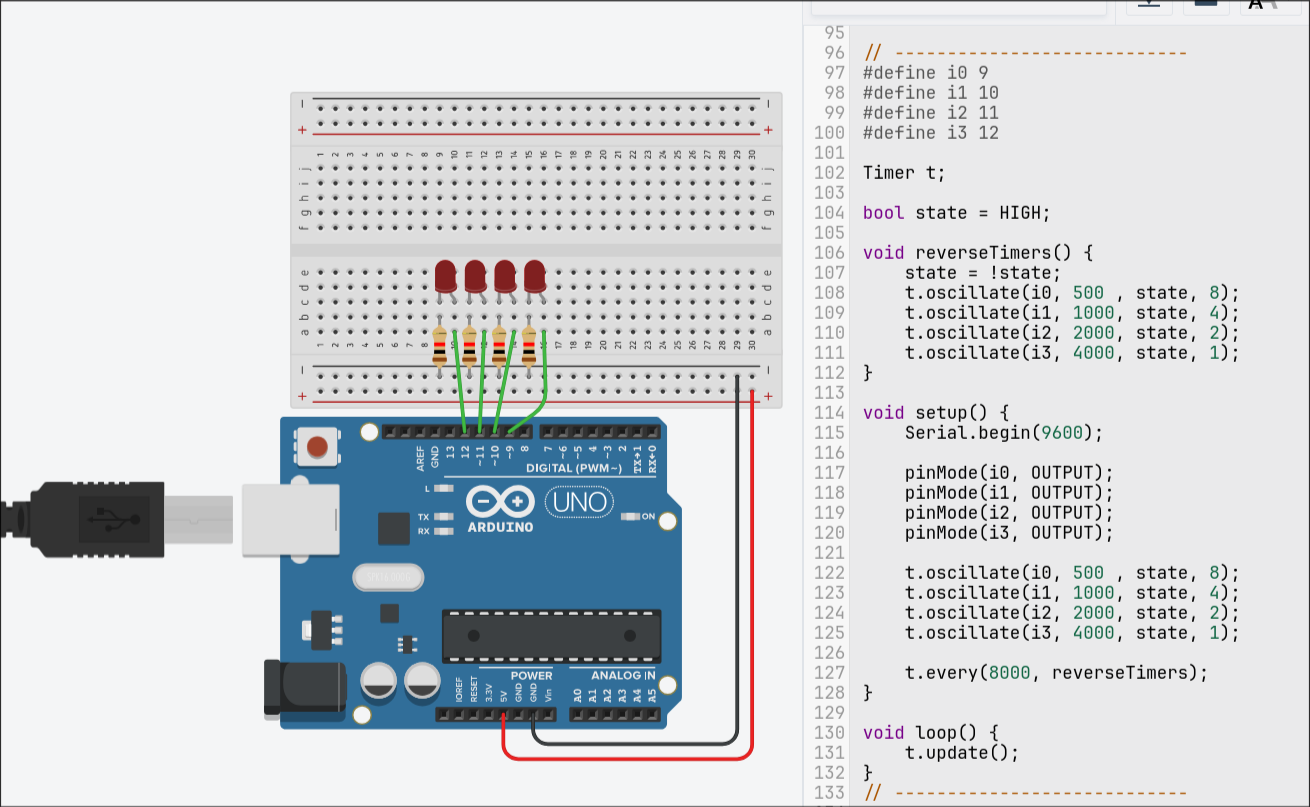
\includegraphics[width=0.8\textwidth]{tc3.png}
    \caption{Tinkercad Simulation Screenshot}
\end{figure}

\subsection{Hardware Setup Photograph}
\begin{figure}[H]
    \centering
    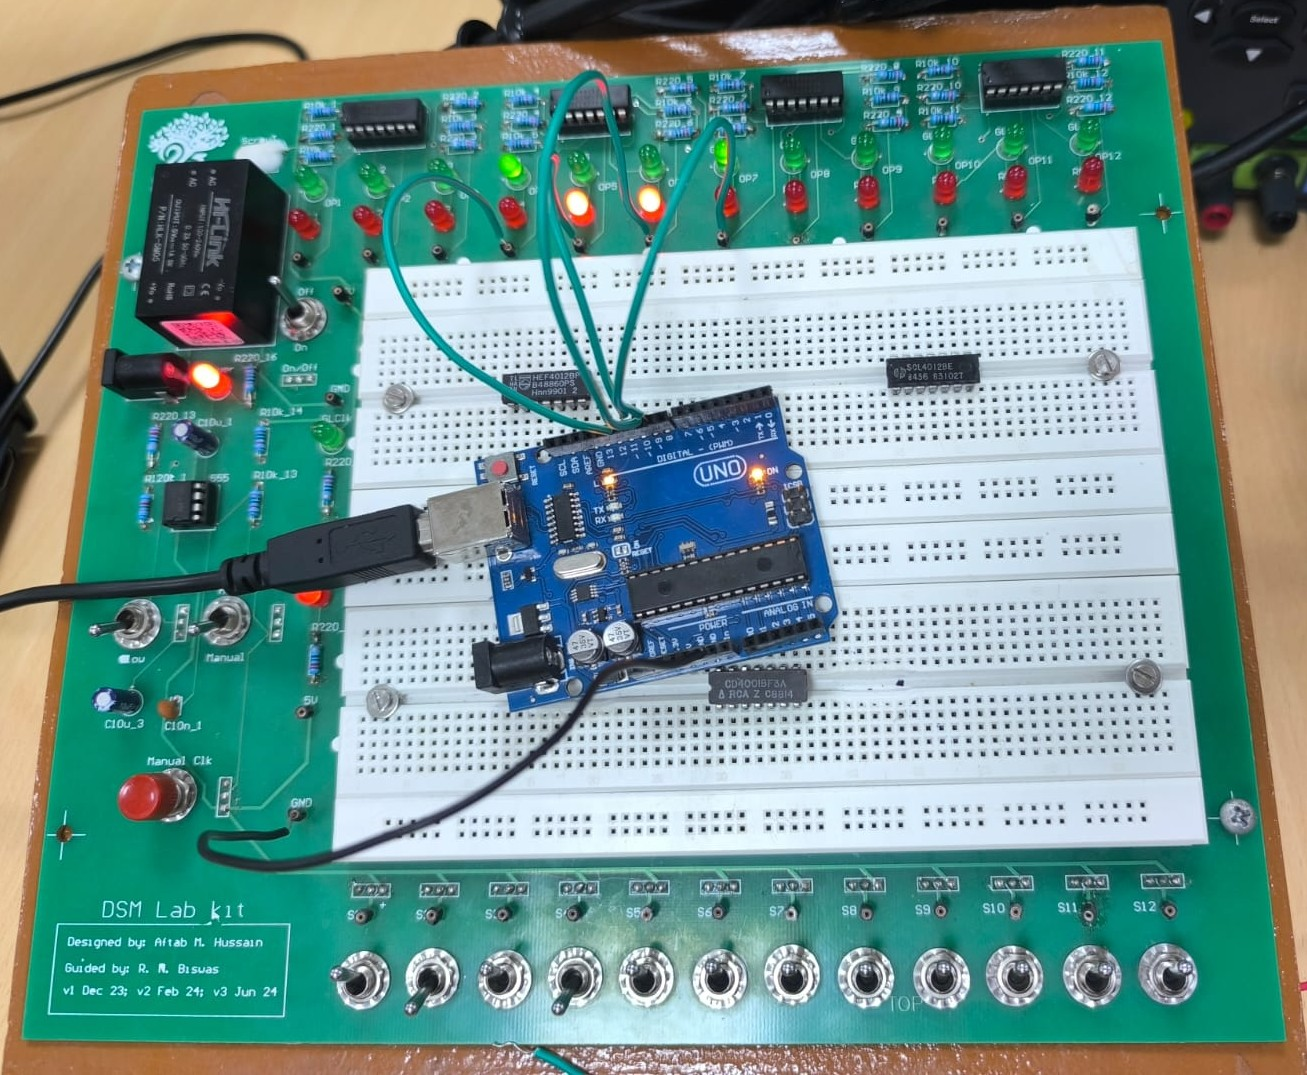
\includegraphics[width=0.6\textwidth]{lab3.jpeg}
    \caption{Hardware Setup for 4-bit Up-Down Counter}
\end{figure}

\subsection{Conclusion}
A 4-bit up-down counter was built using Arduino. $up \rightarrow down \rightarrow up$ cycle from 0 to 15 was verified.

\end{document}